
\chapter{2. Linear PDEs: a structured grid example}

We start with the Poisson problem because it is the right place to start.  Though it is a cliche in applied mathematics, in solving it we will use key parts of \PETSc: build a structured grid using a \PETSc \pDMDA, assemble a \pMat and some \pVecs in parallel on this grid, and solve in parallel using a \pKSP object.

\section{A Poisson problem on a square domain}

The \emph{Laplacian}
    $$\grad^2 u = \Div(\grad u) = \frac{\partial^2 u}{\partial x^2} + \frac{\partial^2 u}{\partial y^2}$$
of a function $u(x,y)$ almost always appears in a mathematical model because the quantity $u$ is conserved in some sense, and because of an assumption that the gradient $\grad u$ is, up to a coefficient, the flux of $u$ \citep{Ockendonetal2003}.  The divergence ``$\Div$'' factor arises from a connection between a flux integral over a closed surface and an integral over the interior of that surface, namely the divergence (Gauss-Green) theorem \citep[Appendix C]{Evans}.

In the \emph{Poisson equation} the Laplacian of $u$ is equal to a known function.  We will not just solve this one equation on a finite region, however.  We solve a \emph{Poisson problem} including boundary conditions, and the whole problem determines a solution which we will approximate numerically.  Let $\mathcal{S}$ be the open unit square $(0,1)\times(0,1)$.  The following is our Poisson problem for this Chapter;  see Figure \ref{fig:unitsquare}:
\begin{marginfigure}
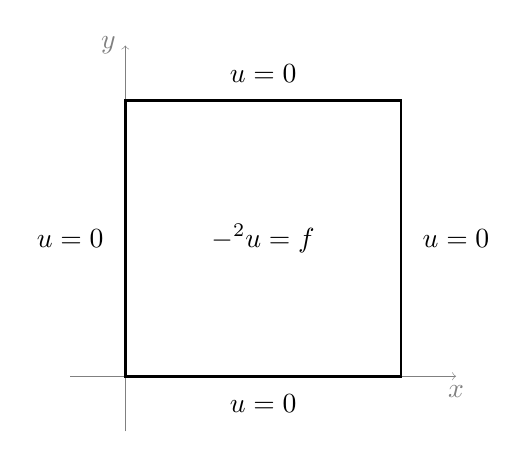
\begin{tikzpicture}[scale=3.5]
  \draw[->,gray,very thin] (-0.2,0.0) -- (1.2,0.0) node[below] {$x$};
  \draw[->,gray,very thin] (0.0,-0.2) -- (0.0,1.2) node[left] {$y$};
  \draw[line width=1.0pt] (0.0,0.0) -- (0.0,1.0) -- (1.0,1.0) -- (1.0,0.0) -- cycle;
  \node at (0.5,0.5) {$- \grad^2 u = f$};
  \node at (0.5,-0.1) {$u = 0$};
  \node at (0.5,1.1) {$u = 0$};
  \node at (-0.2,0.5) {$u = 0$};
  \node at (1.2,0.5) {$u = 0$};
\end{tikzpicture}
\caption{Our first, simple goal is to solve the Poisson equation on the unit square $\mathcal{S}$, with homogeneous Dirichlet boundary conditions.}
\label{fig:unitsquare}
\end{marginfigure}
\begin{align}
- \grad^2 u &= f \quad \text{ on } \mathcal{S}, \label{poissonsquare} \\
u &= 0 \quad \text{ on } \partial \mathcal{S}. \notag
\end{align}
The boundary of the unit square, denoted ``$\partial\mathcal{S}$'', is simply the union of four (closed) line segments.  The boundary conditions $u=0$ are called ``\emph{homogeneous Dirichlet}.''

The Poisson problem can model the electrostatic potential, the equilibrium distribution from certain random walks, the distribution of temperature in a conducting object at steady state, and many other other physical phenomena.  For example, in the context of heat conduction Fourier's law says $\bq = -k \grad u$, where $k$ is approximately constant if the variation in $u$ is not too large.  Conservation of energy for a solid says $c\rho \partial u/\partial t = - \Div\bq + f$ if $f$ describes a heat source within the domain.  At steady state these facts combine to give $0 = k \grad^2 u + f$, that is, Poisson's equation \eqref{poissonsquare}.  Holding the temperature fixed at zero along the boundary completes the problem.

For this chapter we will suppose that $f(x,y)$ is continuous and bounded on $\mathcal{S}$, so that we can compute its pointwise values.  With our homogeneous Dirichlet boundary conditions, and the assumptions on $f$, standard theory says that $u(x,y)$ exists and is continuous on the closed square $\overline{\mathcal{S}}$ \citep[Theorem 6 in section 5.6]{Evans}.\sidenote{A classical approach to showing existence starts by solving problem \eqref{poissonsquare} by Fourier series.  If $f$ is square-integrable then the coefficients $\hat f$ are square-integrable (Parseval's equality).  Because the Laplacian is elliptic and second-order, the coefficients $\hat u$ are square-integrable even when multiplied by the frequency squared.  By Cauchy-Schwarz, the Fourier series for $u$ is the limit of a sequence of continuous functions on $\overline{\mathcal{S}}$ which converge uniformly, so $u\in C^0(\overline{\mathcal{S}})$.}  Thus there is no ambiguity in the boundary condition ``$u=0$ on $\partial \mathcal{S}$,'' and also we can sensibly discuss the pointwise values $u(x,y)$.

Without any boundary conditions, the Poisson equation $-\grad^2 u = f$ alone is not a well-posed problem because if $u$ is a solution then $v=u+C$ is also a solution for any constant $C$.  (In fact there are constant solutions $w=C$ and many, many more to the Laplace equation $-\grad^2 w = 0$ on $\mathcal{S}$.)  However, with the Dirichlet boundary conditions in \eqref{poissonsquare}, the solution is unique if it exists \citep[Theorem 5 in section 2.2]{Evans}; \citep[subsection 5.2.1]{Ockendonetal2003}.


%\clearpage

\section{A finite difference method: build the grid}

Because \eqref{poissonsquare} is a linear problem, finite-dimensional approximations of it are simply linear systems.  The finite-dimensional approximation in this Chapter comes from applying a \emph{finite difference} (FD) method.  In Chapter 3 we will apply a finite element approach instead.

\begin{marginfigure}
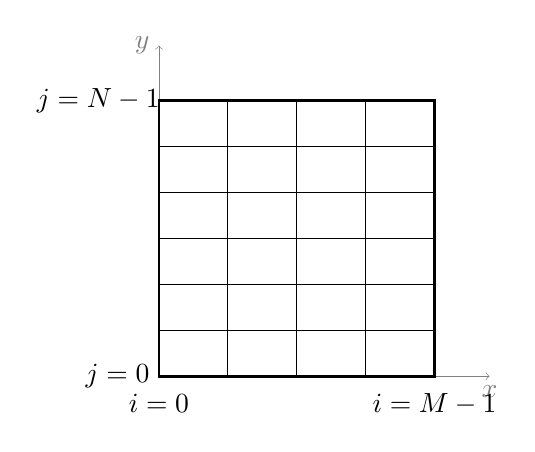
\begin{tikzpicture}[scale=3.5]
  \draw[->,gray,very thin] (0.0,0.0) -- (1.2,0.0) node[below] {$x$};
  \draw[->,gray,very thin] (0.0,0.0) -- (0.0,1.2) node[left] {$y$};
  \draw[line width=1.0pt] (0.0,0.0) -- (0.0,1.0) -- (1.0,1.0) -- (1.0,0.0) -- cycle;
  \node at (0.0,-0.1) {$i=0$};
  \node at (1.0,-0.1) {$i=M-1$};
  \node at (-0.15,0.0) {$j=0$};
  \node at (-0.22,1.0) {$j=N-1$};
  \draw[xstep=0.25,ystep=0.166667,black,thin] (0.0,0.0) grid (1.0,1.0);
\end{tikzpicture}
\caption{A grid on the unit square $\mathcal{S}$, with $M=5$ and $N=7$.}
\label{fig:unitsquaregrid}
\end{marginfigure}

To start our FD method we put a \emph{structured grid} of $MN$ points on the unit square, as in Figure \ref{fig:unitsquaregrid}, with spacing $h_x=1/(M-1)$ and $h_y=1/(N-1)$ in the two directions.  The grid locations are $x_i = i\, h_x$ for $i = 0,1,\dots,M-1$ and $y_j = j\, h_y$ and $j=0,1,\dots,N-1$.

The construction of such a two-dimensional (2D) grid, and the distribution of it across processors, will be our first new idea from \PETSc, beyond the basics in Chapter 1.  Consider the lines of code in Figure \ref{code:dmdacreatetwod}.  They create a \PETSc \pDM object\sidenote{``\pDM'' might stand for ``data management'', but perhaps ``distributed mesh'' is better.} for a grid like Figure \ref{fig:unitsquaregrid}.

\clearpage
\cinputraw{dmdacreate2d.frag}{extract from c2poisson.c}{An example of creating a 2D \pDMDA.}{}{//START}{//STOP}{code:dmdacreatetwod}

A \pDM is an abstract type for describing the topology (i.e.~connectedness) of a grid, \emph{and} the way it is distributed across \MPI processes, \emph{and} the way each process can access data from its neighbors.  The specific variable \texttt{da} in Figure \ref{code:dmdacreatetwod} has type ``\pDMDA'', which is the subclass of \pDM s which are structured grids.

The Figure \ref{code:dmdacreatetwod} code will appear in \texttt{c2poisson.c} below, which solves Poisson's problem.  For now, if we do
\begin{Verbatim}[fontsize=\small]
  make c2poisson
  mpiexec -n 4 ./c2poisson -da_grid_x 5 -da_grid_y 7
\end{Verbatim}
then a structured grid will be distributed across the four processes exactly as in Figure \ref{fig:unitsquaregridparallel}.  Neither $M=5$ nor $N=7$ is divisible by two in this case, but \PETSc distributes the four ranks across the $MN=35$ nodes (grid points) as uniformly as possible given that each processor owns a rectangular subgrid.  In fact, the rank $0$ process has the most nodes (12) and rank $3$ has the least (6), so the load is only uniform within a factor of two, but larger grids will be better load-balanced.  \PETSc does the best it can.

\begin{marginfigure}
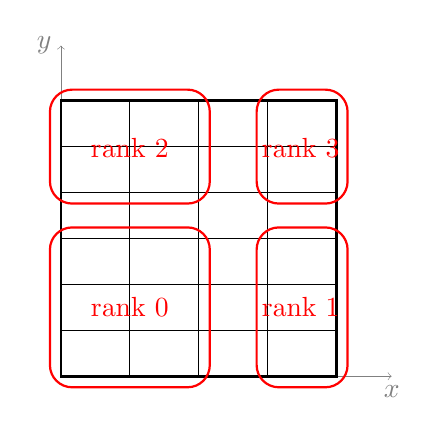
\begin{tikzpicture}[scale=3.5]
  \draw[->,gray,very thin] (0.0,0.0) -- (1.2,0.0) node[below] {$x$};
  \draw[->,gray,very thin] (0.0,0.0) -- (0.0,1.2) node[left] {$y$};
  \draw[line width=1.0pt] (0.0,0.0) -- (0.0,1.0) -- (1.0,1.0) -- (1.0,0.0) -- cycle;
  \draw[xstep=0.25,ystep=0.166667,black,thin] (0.0,0.0) grid (1.0,1.0);
  \draw[thick,rounded corners=8pt,color=red]
(-0.04,-0.04) -- (-0.04,0.54) -- (0.54,0.54) -- (0.54,-0.04) -- cycle;
  \node[color=red] at (0.25,0.25) {rank $0$};
  \draw[thick,rounded corners=8pt,color=red]
(0.71,-0.04) -- (0.71,0.54) -- (1.04,0.54) -- (1.04,-0.04) -- cycle;
  \node[color=red] at (0.87,0.25) {rank $1$};
  \draw[thick,rounded corners=8pt,color=red]
(-0.04,0.626667) -- (-0.04,1.04) -- (0.54,1.04) -- (0.54,0.62667) -- cycle;
  \node[color=red] at (0.25,0.83) {rank $2$};
  \draw[thick,rounded corners=8pt,color=red]
(0.71,0.626667) -- (0.71,1.04) -- (1.04,1.04) -- (1.04,0.626667) -- cycle;
  \node[color=red] at (0.87,0.83) {rank $3$};
\end{tikzpicture}
\caption{The same grid as in Figure \ref{fig:unitsquaregrid}, distributed across four \MPI processes (i.e.~with \texttt{rank} $\in \{0,1,2,3\}$) automatically by \texttt{DMDACreate2d()}.}
\label{fig:unitsquaregridparallel}
\end{marginfigure}

The fifth and sixth arguments ``\texttt{-10}'' to \texttt{DMDACreate2d()} in Figure \ref{code:dmdacreatetwod} are used to set default dimensions $M=10$ and $N=10$.  We have seen that these defaults are overridden by runtime options \texttt{-da\_grid\_x} and \texttt{-da\_grid\_y}.  However, if we do this,
 \begin{Verbatim}[fontsize=\small]
  mpiexec -n 4 ./c2poisson
\end{Verbatim}
then a structured grid will be distributed across the four processes as in Figure \ref{fig:unitsquaregrideight}, with each rank owning 25 nodes.  \PETSc itself can show the parallel layout by calling
\begin{Verbatim}[fontsize=\small]
  mpiexec -n 4 ./c2poisson -dm_view
\end{Verbatim}
or
\begin{Verbatim}[fontsize=\small]
  mpiexec -n 4 ./c2poisson -dm_view draw -draw_pause 2
\end{Verbatim}
The latter version shows the grid graphically, for two seconds.

\begin{marginfigure}
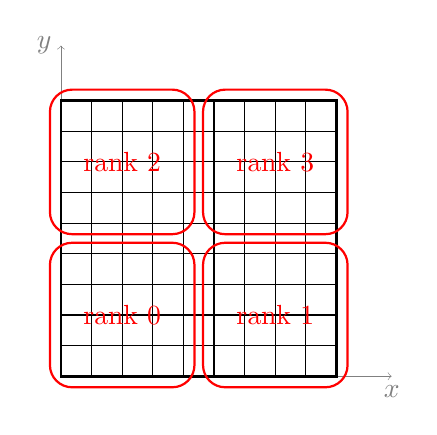
\begin{tikzpicture}[scale=3.5]
  \draw[->,gray,very thin] (0.0,0.0) -- (1.2,0.0) node[below] {$x$};
  \draw[->,gray,very thin] (0.0,0.0) -- (0.0,1.2) node[left] {$y$};
  \draw[line width=1.0pt] (0.0,0.0) -- (0.0,1.0) -- (1.0,1.0) -- (1.0,0.0) -- cycle;
  \pgfmathsetmacro\ninth{1.0/9.0}
  \draw[xstep=\ninth,ystep=\ninth,black,thin] (0.0,0.0) grid (1.0,1.0);
  \pgfmathsetmacro\dd{0.04}
  \pgfmathsetmacro\od{1.04}
  \pgfmathsetmacro\ap{4*\ninth + 0.04}
  \pgfmathsetmacro\bm{5*\ninth - 0.04}
  \pgfmathsetmacro\amid{2*\ninth}
  \pgfmathsetmacro\bmid{7*\ninth}
  \draw[thick,rounded corners=8pt,color=red]
    (-\dd,-\dd) -- (-\dd,\ap) -- (\ap,\ap) -- (\ap,-\dd) -- cycle;
  \node[color=red] at (\amid,\amid) {rank $0$};
  \draw[thick,rounded corners=8pt,color=red]
    (\bm,-\dd) -- (\od,-\dd) -- (\od,\ap) -- (\bm,\ap) -- cycle;
  \node[color=red] at (\bmid,\amid) {rank $1$};
  \draw[thick,rounded corners=8pt,color=red]
    (-\dd,\bm) -- (\ap,\bm) -- (\ap,\od) -- (-\dd,\od) -- cycle;
  \node[color=red] at (\amid,\bmid) {rank $2$};
  \draw[thick,rounded corners=8pt,color=red]
    (\bm,\bm) -- (\od,\bm) -- (\od,\od) -- (\bm,\od) -- cycle;
  \node[color=red] at (\bmid,\bmid) {rank $3$};
\end{tikzpicture}
\caption{An $M=10$ by $N=10$ grid distributed by \texttt{DMDACreate2d()} across four \MPI processes.}
\label{fig:unitsquaregrideight}
\end{marginfigure}

To explain the other options to \texttt{DMDACreate2d()} used in Figure \ref{code:dmdacreatetwod}, we quote the \PETSc manual pages description of that method:

\clearpage
\noindent\hrulefill
\begin{Verbatim}[fontsize=\small]
DMDACreate2d(MPI_Comm comm, DMBoundaryType bx, DMBoundaryType by,
  DMDAStencilType stype, PetscInt M, PetscInt N, PetscInt m, PetscInt n,
  PetscInt dof, PetscInt s, const PetscInt lx[], const PetscInt ly[],
  DM *da)
\end{Verbatim}
where
\small
\begin{itemize}[align=left]
\item[\texttt{comm}]   MPI communicator \\
\item[\texttt{bx,by}]  type of ghost nodes the array have; use one of \texttt{DM\_BOUNDARY\_NONE, DM\_BOUNDARY\_GHOSTED, DM\_BOUNDARY\_PERIODIC} \\
\item[\texttt{stype}] stencil type; use either \texttt{DMDA\_STENCIL\_BOX} or \texttt{DMDA\_STENCIL\_STAR} \\
\item[\texttt{M,N}]	   global dimension in each direction of the array; use \texttt{-M} and or \texttt{-N} to indicate that it may be set to a different value from the command line with \texttt{-da\_grid\_x <M> -da\_grid\_y <N>} \\
\item[\texttt{m,n}]   corresponding number of processors in each dimension (or \texttt{PETSC\_DECIDE} to have calculated) \\
\item[\texttt{dof}]     number of degrees of freedom per node \\
\item[\texttt{s}]       stencil width \\
\item[\texttt{lx,ly}]  arrays containing the number of nodes in each cell along the x and y coordinates, or \texttt{NULL}; if non-null, these must be of length as m and n, and the corresponding m and n cannot be \texttt{PETSC\_DECIDE}; the sum of the \texttt{lx[]} entries must be M, and the sum of the \texttt{ly[]} entries must be N \\
\item[\texttt{da}]      output: the resulting distributed array object 
\end{itemize}
\normalsize
\noindent\hrulefill
\medskip

In Figure \ref{code:dmdacreatetwod}, the first argument is a serial or parallel \MPI communicator.  In the second and third arguments we have used ``\texttt{DM\_BOUNDARY\_NONE}'' because our Dirichlet boundary condition does not require communication to the next process' domain, nor periodic wrapping.  In the fourth argument we use \texttt{DMDA\_STENCIL\_STAR} because only cardinal neighbors of a grid point are used when forming the matrix; we will address the FD ``stencil'' below.  As already noted, the fifth and sixth arguments set $M=10,N=10$ as override-able grid defaults.  In the next two arguments we indeed use ``\texttt{PETSC\_DECIDE}'' to have \PETSc parallel-decompose our grid according to the size of (i.e.~number of processes in) the \MPI communicator.  The next two arguments, in the ninth and tenth positions, say that our PDE is scalar (\texttt{dof}$=1$) and that the FD method only needs one neighbor in each direction (\texttt{s}$=1$).  The next two arguments are \texttt{NULL} because we are \emph{not} telling \PETSc how to distribute processes over the grid; it \texttt{DECIDE}s for itself.  Finally, the \pDMDA object is created as an output.

The call to \texttt{DMDASetUniformCoordinates()} in Figure \ref{code:dmdacreatetwod} sets the domain to be $[0,1]\times[0,1]$.  The last two arguments are ignored in this case but would set limits on the third dimension in 3D.

To wrap up our coverage of creating grids, the standard \PETSc view of what \pDM s ``look like'' is in Figure \ref{fig:petscghostvalues}.  On the left is a version of what we have done in the code in Figure \ref{code:dmdacreatetwod}, namely create a structured grid \pDM.  The one shown in Figure \ref{fig:petscghostvalues} has \texttt{DMDA\_STENCIL\_BOX} stencil type, unlike ours.  On the right is an unstructured grid, of the type created in Chapter 3 for the finite element method.  In both cases the figure shows nodes owned by a given process (red ``local'' nodes) and those other nodes that are accessible by the local process (blue ``ghost'' nodes).  We will see such local/ghost node types in all examples in this book.

\begin{figure}
\includegraphics[width=\textwidth]{petscghostvalues}
\caption{\PETSc's parallel decomposition of structured and unstructured grids, showing owned (``local'') and accessible (``ghost'') nodes for one process.}
\label{fig:petscghostvalues}
\end{figure}


\section{A finite difference method: assemble the linear system}

Recall we were trying to approximate PDE problem \eqref{poissonsquare}.  Having built a structured grid we can now return to the FD method.

By a well-known Taylor's theorem argument \citep{MortonMayers}, for any function $F(x)$ which is sufficiently smooth, we have
    $$F''(x) = \frac{F(x+h) - 2 F(x) + F(x-h)}{h^2} + O(h^2)$$
as $h$ goes to zero.  This formula, applied to partial derivatives, will give an approximation of the Laplacian in problem \eqref{poissonsquare}.

Let $U_{i,j}$ be the gridded approximation to the exact value $u(x_i,y_j)$ of the solution $u$,\sidenote{This is an important sentence!  We \emph{compute} values $U_{i,j}$ from the finite difference equations.  We generally \emph{don't know} the values of the exact solution on the grid, namely $u(x_i,y_j)$.  Of course we want the former to be close to the latter.}  and also denote $f_{i,j} = f(x_i,y_j)$.  Then we have this FD approximation to problem \eqref{poissonsquare}:
\begin{equation}
- \frac{U_{i+1,j} - 2 U_{i,j} + U_{i-1,j}}{h_x^2} - \frac{U_{i,j+1} - 2 U_{i,j} + U_{i,j-1}}{h_y^2} = f_{i,j}. \label{poissonsquareFDearly}
\end{equation}
Equation \eqref{poissonsquareFDearly} applies for all of the interior points where $1 \le i \le M-2$ and $1 \le j \le N-2$.  The boundary conditions in \eqref{poissonsquare} become
\begin{align}
U_{0,j} &= 0, \label{poissonsquareFDbcs} \\
U_{M-1,j} &= 0, \notag \\
U_{i,0} &= 0, \notag \\
U_{i,N-1} &= 0, \notag
\end{align}
for all $i,j$.

Equations \eqref{poissonsquareFDearly} and \eqref{poissonsquareFDbcs} form a linear system in which we choose to treat all $MN$ locations on the grid as unknowns.  Surprisingly, perhaps, there are two nontrivial observations to make about this system.  

First, the equations have very different ``scaling''.  For example, if $M=N=1001$ so that $h_x=h_y=0.001$ then the coefficient of $U_{i,j}$ in \eqref{poissonsquareFDearly} is $4/(.001)^2 = 4 \times 10^6$, where as the coefficients of $U_{i,j}$ along the boundary in \eqref{poissonsquareFDbcs} are equal to 1.  For this reason we multiply equation \eqref{poissonsquareFDearly} by the grid cell area $h_x h_y$ to get
\begin{align}
&\left(2 \frac{h_y}{h_x} + 2 \frac{h_x}{h_y}\right) U_{i,j} - \frac{h_y}{h_x}\left(U_{i+1,j} + U_{i-1,j}\right)  - \frac{h_x}{h_y}\left(U_{i,j+1} + U_{i,j-1}\right) \label{poissonsquareFD} \\
&\qquad = h_x h_y f_{i,j}. \notag
\end{align}
While one might complain about this form's appearance, note that in the $h_x=h_y$ case, regardless of whether the grid is fine or coarse, the equation is
    $$4 U_{i,j} - U_{i+1,j} - U_{i-1,j} - U_{i,j+1} - U_{i,j-1}  = h_x h_y f_{i,j},$$
with coefficients of size one.

Second, \eqref{poissonsquareFDearly} or \eqref{poissonsquareFD} can be interpreted to give a symmetric matrix.  FIXME: BUILD MATRIX AND REPEAT IT IS SYMMETRIC


\begin{marginfigure}
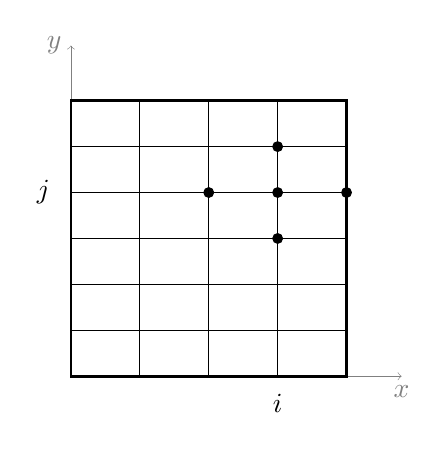
\begin{tikzpicture}[scale=3.5]
  \draw[->,gray,very thin] (0.0,0.0) -- (1.2,0.0) node[below] {$x$};
  \draw[->,gray,very thin] (0.0,0.0) -- (0.0,1.2) node[left] {$y$};
  \draw[line width=1.0pt] (0.0,0.0) -- (0.0,1.0) -- (1.0,1.0) -- (1.0,0.0) -- cycle;
  \node at (0.75,-0.1) {$i$};
  \node at (-0.1,0.666667) {$j$};
  \filldraw (0.50,0.666667) circle (0.5pt);
  \filldraw (0.75,0.666667) circle (0.5pt);
  \filldraw (1.00,0.666667) circle (0.5pt);
  \filldraw (0.75,0.5) circle (0.5pt);
  \filldraw (0.75,0.833333) circle (0.5pt);
  \draw[xstep=0.25,ystep=0.166667,black,thin] (0.0,0.0) grid (1.0,1.0);
\end{tikzpicture}
\caption{A stencil, shown on the grid, at $i=3$ and $j=4$.}
\label{fig:unitsquaregridstencil}
\end{marginfigure}

\cinput{structuredlaplacian.c}{Fill matrix entries using \texttt{MatSetValuesStencil}.}{//CREATEMATRIX}{//ENDCREATEMATRIX}{code:structuredlaplacian}

\cinputpart{c2poisson.c}{The right side of equation \eqref{poissongridsystem} comes from differentiating the exact solution, which this method also computes.}{I}{//RHS}{//ENDRHS}{code:ctwopoissonrhs}

\cinputpart{c2poisson.c}{Set up \pDMDA \texttt{da} and \pMat \texttt{A} objects, and assemble the latter by calling \texttt{formlaplacian()}.}{II}{//CREATE}{//ENDCREATE}{code:ctwopoissoncreate}

\cinputpart{c2poisson.c}{Solve using \pKSP, and report on solution.}{III}{//SOLVE}{//ENDSOLVE}{code:ctwopoissonsolve}

\section{Runtime control of linear solver}

FIXME: basic Krylov theory

\section{Time-dependent heat equation}

FIXME: we WON'T do explicit, but it would look like ...

FIXME: use TS for backward-euler
